\documentclass[12pt]{article}
\usepackage[T1]{fontenc}
\usepackage{framed}
\usepackage[margin=1in,top=0.5in]{geometry}
\usepackage{graphicx}
\usepackage{longtable}
\usepackage{moreverb}
\usepackage{multirow}
\thispagestyle{empty}
\begin{document}
\setlength{\parindent}{0pt}

\begin{framed}
Sol Boucher and Evan Klei \hfill CSCI-453-01 \hfill 04/28/14 \\
\vspace{6pt} \\
\centerline{\textbf{\huge FabComp: Hardware specification}}
\end{framed}

\section{Hardware}
The computer is composed of a largely isolated data unit and control unit, which are only connected by a couple of direct buses.

\subsection{Data path}
All components of the data path have both 16-bit word size and address length.
They are connected as such:

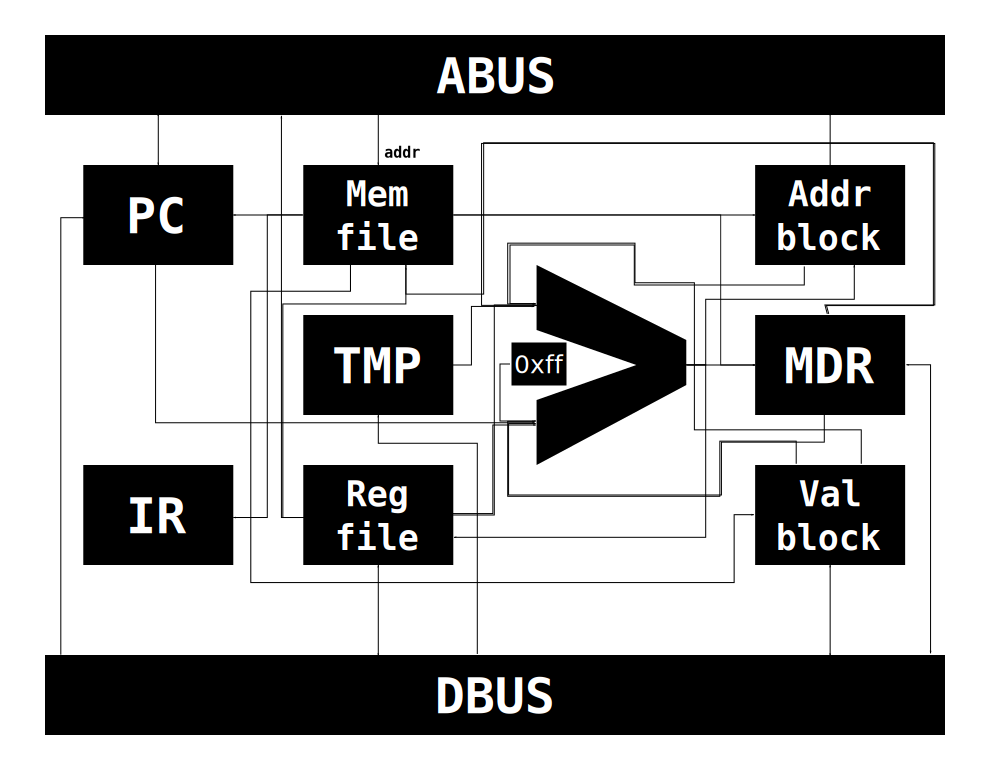
\includegraphics[width=\textwidth]{datapath}

The system's storage components adhere to these specifications:

\vspace{6pt}
\begin{tabular}{| c | c | l |}
\hline
\multicolumn{3}{| c |}{data path storage objects} \\
\hline
name & type & purpose \\
\hline
PC & counter register & program counter \\
IR & shift register & instruction register \\
MDR & shift register & main data register \\
TMP & register & temporary register \\
Mem & memory & main memory (program and data) \\
Reg & 16-register bank & general-purpose registers (\textit{see} ISA document, section 5) \\
Val & 3-register bank & storage of immediate values \\
Addr & 3-register bank & storage of effective addresses \\
\hline
\end{tabular}

\subsection{Control path}
The word size and address widths within the control path are component-specific:

\vspace{6pt}
\begin{tabular}{| c | c | c | l |}
\hline
\multicolumn{4}{| c |}{control path storage objects} \\
\hline
name & type & word size & purpose \\
\hline
uPC & counter register & 12-bit & microprogram counter \\
uIR & register & 16-bit & microinstruction register \\
cntl & 3-register bank & 5-bit & operand control flags \\
tmp & register & 5-bit & temporary control flags \\
i & counter register & 2-bit & track current working operand \\
regshift & shift register & 16-bit & transfer register IDs from data path \\
uSP & counter register & 2-bit & micro--stack pointer \\
uStack & 3-register bank & 12-bit & subprocedure return addresses \\
uMem & memory & 16-bit data, 12-bit addr & contains hardcoded microprogram \\
uJumpTab & memory & 16-bit data, 5-bit addr & hardcoded jump table \\
\hline
\end{tabular}

\includegraphics[width=\textwidth]{controlpath}

The 3 control registers are used to represent the source and destination operand locations:

\vspace{6pt}
\begin{tabular}{| c | c | l |}
\hline
\multicolumn{3}{| c |}{control registers encoding/flags} \\
\hline
msb & trailing bits & significance \\
\hline
0 & 4-bit register identifier & this operand/destination is located in the specified GPR \\
1 & 0000 & this operand is not used by the current operation \\
1 & 0001 & this operand is located in register Val[1] \\
1 & 0010 & this operand is located in register Val[2] \\
1 & 0011 & this operand is located in the MDR \\
1 & 0100 & this operand/destination is located at memory address Addr[0] \\
1 & 0101 & this operand is located at memory address Addr[1] \\
1 & 0110 & this operand is located at memory address Addr[2] \\
\hline
\end{tabular}

\section{Register transfer language}
Here is the sequence of hardware actions performed by each phase of instruction processing:

% BEGIN RTL
\subsection{Fetch phase}
\begin{verbatimtab}
IR <- Mem[PC] # the instruction word
PC <- PC + 1
\end{verbatimtab}

\subsection{Decode phase}
\begin{verbatimtab}
i <- 00
while i != 11 do
	if i != 00 AND IR(imm)(i) = 1 then
		Val[i] <- Mem[PC]
		cntl[i] <- 10000 | i
		PC <- PC + 1
	elif IR(ami) = 00 then
		cntl[i] <- 10000
	elif IR(ami) = 01 or 10 then
		Addr[i] <- Mem[PC]
		cntl[i] <- 10100 | i
		PC <- PC + 1
	elif IR(ami) = 11 then
		MDR <- Mem[PC] # the R-type immediate word
		cntl[i] <- 10100 | i
		PC <- PC + 1
		if MDR(sam) = 000 then # register value
			cntl[i] <- 00000 | MDR(reg0)
		elif MDR(sam) = 001 then # register indirect
			Addr[i] <- Reg[MDR(reg0)]
		elif MDR(sam) = 010 then # scaled
			Val[i] <- MDR
			MDR <- Mem[PC] # the S-type immediate
			PC <- PC + 1
			MDR <- MDR >> 8
			Addr[i] <- Reg[Val[i](reg1)] << MDR
			Addr[i] <- Addr[i] + Reg[Val[i](reg0)]
		elif MDR(sam) = 011 then # doubly scaled
			Val[i] <- MDR
			MDR <- Mem[PC]
			TMP <- MDR
			PC <- PC + 1
			MDR <- MDR >> 8
			Addr[i] <- Reg[Val[i](reg1)] << MDR
			Addr[i] <- Reg[Val[i](reg0)] + Addr[i]
			MDR <- Mem[Addr[i]]
			Addr[i] <- MDR
			MDR <- TMP & 0xff
			MDR <- Reg[Val[i](reg2)] << MDR
			Addr[i] <- MDR + Addr[i]
		elif MDR(sam) = 100 then # auto increment
			Val[i] <- MDR
			Addr[i] <- Reg[Val[i](reg0)]
			Reg[Val[i](reg0)] <- Reg[Val[i](reg0)] + 1
		elif MDR(sam) = 101 then # auto decrement
			Val[i] <- MDR
			Addr[i] <- Reg[Val[i](reg0)]
			Reg[Val[i](reg0)] <- Reg[Val[i](reg0)] - 1
		elif MDR(sam) = 110 then # scaled displacement
			Val[i] <- MDR
			MDR <- Mem[PC] # the S-type immediate
			PC <- PC + 1
			MDR <- MDR >> 8
			Addr[i] <- Reg[Val[i](reg0)] << MDR
			MDR <- Mem[PC] # the I-type immediate
			PC <- PC + 1
			Addr[i] <- MDR + Addr[i]
		elif MDR(sam) = 111 then # doubly scaled displacement
			Val[i] <- MDR
			MDR <- Mem[PC] # the S-type immediate
			PC <- PC + 1
			TMP <- MDR
			MDR <- MDR >> 8
			Addr[i] <- Reg[Val[i](reg0)] << MDR
			MDR <- Mem[PC] # the I-type immediate
			PC <- PC + 1
			Addr[i] <- MDR + Addr[i]
			MDR <- Mem[Addr[i]]
			Addr[i] <- MDR
			MDR <- TMP & 0xff
			MDR <- Reg[Val[i](reg1)] << MDR
			Addr[i] <- Addr[i] + MDR
		fi
	fi
	i <- i + 1
done

i <- 00
while i != 11 do
	if IR(ami) = 10 then # PC-relative
		Addr[i] <- PC + Addr[i]
	fi
done
\end{verbatimtab}

\subsection{Memory Load}
\begin{verbatimtab}
if cntl[1](4) = 1 AND cntl[1](2) = 1 then
	Val[1] <- Mem[Addr[1]]
	cntl[1](2) <- 0
fi
if cntl[2](4) = 1 AND cntl[2](2) = 1 then
	Val[2] <- Mem[Addr[2]]
	cntl[2](2) <- 0
fi
\end{verbatimtab}

\subsection{Execute}
\begin{verbatimtab}
# call function described by entry IR(opc) of an off-memory uJumpTable

halt:
	# bail out
and:
	# call validator_one
	MDR <- op1 & op2
	# return
or:
	# call validator_one
	MDR <- op1 | op2
	# return
xor:
	# call validator_one
	MDR <- op1 ^ op2
	# return
lsft:
	# call validator_one
	MDR <- op1 << op2
	# return
nand:
	# call validator_one
	# call and
	cntl[1] <- 10011
	cntl[2] <- 10000
	# call not
	# return
nor:
	# call validator_one
	# call or
	cntl[1] <- 10011
	cntl[2] <- 10000
	# call not
	# return
xnor:
	# call validator_one
	# call xor
	cntl[1] <- 10011
	cntl[2] <- 10000
	# call not
	# return
rsft:
	# call validator_one
	MDR <- op1 >> op2
	# return
# logical goes here
# logical goes here
# logical goes here
rasft:
	# call validator_one
	MDR <- op1 >>> op2
	# return
# logical goes here
# logical goes here
# logical goes here
slt:
	# call validator_one
	# call sub
	if MDR(15) = 1
		MDR <- 1
	else
		MDR <- 0
	fi
	# return
sgt:
	# call validator_one
	MDR <- op2 - op1
	if MDR(15) = 1
		MDR <- 1
	else
		MDR <- 0
	fi
	# return
seq:
	# call validator_one
	# call sub
	if MDR = 0
		MDR <- 1
	else
		MDR <- 0
	fi
	# return
sne:
	# call validator_one
	# call seq
	cntl[1] <- 10011
	cntl[2] <- 10000
	# call not
	# return
sle:
	# call validator_one
	# call sgt
	cntl[1] <- 10011
	cntl[2] <- 10000
	# call not
	# return
sge:
	# call validator_one
	# call slt
	cntl[1] <- 10011
	cntl[2] <- 10000
	# call not
	# return
add:
	# call validator_one
	MDR <- op1 + op2
	# return
sub:
	# call validator_one
	MDR <- op1 - op2
	# return
# compbranch goes here
# compbranch goes here
# compbranch goes here
# compbranch goes here
# compbranch goes here
# compbranch goes here
# validator_three goes here
# validator_three goes here
siz:
	# call validator_four
	if op1 = 0
	   MDR <- 1
	else
	   MDR <- 0
	fi
	# return
snz:
	# call validator_four
	# call siz
	cntl[1] <- 10011
	# call not
	# return
not:
	# call validator_four
	MDR <- ~ op1
	# return
neg:
	# call validator_four
	MDR <- 0 - op1
	# return
# simpbranch goes here
# simpbranch goes here
incr:
	# call validator_six
	MDR <- op0 + 1
	# return
decr:
	# call validator_six
	MDR <- op0 - 1
	# return
jmp:
	# call validator_seven
	PC <- op0
	cntl[0] <- 10011
	# return

jal:
	# call validator_seven
	Reg[15] <- PC
	PC <- op0
	cntl[0] <- 10011
	# return
call:
	# call validator_seven
	# call jal
	Reg[14] <- Reg[14] - 1
	Mem[Reg[14]] <- Reg[15]
	# return
ret:
	# call validator_eight
	cntl[0] <- 01111
	# call jmp
	Reg[14] <- Reg[14] + 1
	# return
move:
	# call validator_nine
	MDR <- op1
	# return

logical: # handles land, lor, lxor, lnand, lnor, lxnor
	# call validator_one
	tmp <- cntl[2]
	cntl[2] <- 10000
	# call siz
	Val[1] <- MDR
	cntl[1] <- tmp
	cntl[2] <- 10000
	# call siz
	cntl[1] <- 10001
	cntl[2] <- 10011
	# call function described by entry IR(opc) - 4 of an off-memory uJumpTable
	# return

compbranch: # handles blt, bgt, beq, bne, ble, bge
	# call validator_two
	# call function described by entry IR(opc) - 8 of an off-memory uJumpTable
	cntl[2] <- 10000
	cntl[1] <- cntl[0]
	# call bnz
	# return

simpbranch: # handles biz, bnz
	# call validator_five
	# call function described by entry IR(opc) - 4 of an off-memory uJumpTable
	if MDR = 1 then
		PC <- op0
	fi
	cntl[0] <- 10011
	# return

validator_one:
	# Check for 2-3 ops
	if cntl[0] = 10000
		# bail out loudly
	fi
	if cntl[1] = 10000 then
		# bail out loudly
	fi
	if cntl[2] = 10000 then
		cntl[2] <- cntl[1]
		cntl[1] <- cntl[0]
	fi
	# return

validator_two:
	# Check for 3 ops, op0 is not a register
	if cntl[0] = 10000 then
		# bail out loudly
	fi
	if cntl[1] = 10000 then
		# bail out loudly
	fi
	if cntl[2] = 10000 then
		# bail out loudly
	fi
	if cntl[0](4) = 0 then
		# bail out loudly
	fi
	# return

validator_three:
	# Kill immediately
	# bail out loudly

validator_four:
	# Check for 1-2 ops, set cntl[1] if it was empty

validator_five:
	# Check for 2 ops, op0 is not a register
	if cntl[0] = 10000 then
		# bail out loudly
	fi
	if cntl[1] = 10000 then
		# bail out loudly
	fi
	if cntl[0](4) = 0 then
		# bail out loudly
	fi
	# return

validator_six:
	# Check for 1 op
	if cntl[0] = 10000 then
		# bail out loudly
	fi
	# return

validator_seven:
	# Check for 1 op, op0 is not a register
	if cntl[0] = 10000 then
		# bail out loudly
	fi
	if cntl[0](4) = 0 then
		# bail out loudly
	fi
	# return

validator_eight:
	# Check for 0 op
	# return

validator_nine:
	# Check for 2 ops
	if cntl[0] = 10000 then
		# bail out loudly
	fi
	if cntl[1] = 10000 then
		# bail out loudly
	fi
	# return
\end{verbatimtab}

\subsection{Writeback}
\begin{verbatimtab}
if cntl[0](4) = 0 then
	Reg[cntl[0](3..0)] <- MDR
elif cntl[0](4) = 1 then
	Mem[Addr[cntl[0](3..0)]] <- MDR
fi
# jump to the very beginning
\end{verbatimtab}
% END RTL

\section{Microinstruction format}
Each microinstruction is encoded as a single word, with one of two possible formats:

\vspace{6pt}
\begin{tabular}{| c | c |}
\hline
\multicolumn{2}{| c |}{C-type word format} \\
\hline
0000 & control points \\
\hline

15 \hfill 12 & 11 \hfill 0 \\
\end{tabular}
\begin{tabular}{| c | c | c |}
\hline
\multicolumn{3}{| c |}{J-type word format} \\
\hline
type & condition & jump index \\
\hline
15 \hfill 12 & 11 \hfill 7 & 6 \hfill 0 \\
\end{tabular}

\subsection{C-type microinstructions}
This microinstruction type is used to set control points and move data around in the data and control paths.
The encoding is entirely vertical and therefore supports no parallelism beyond that encoded into the discrete control point identifiers themselves.

\begin{longtable}{| c | l |}
\hline
\multicolumn{2}{| c |}{control point settings} \\
\hline
encoding & equivalent RTL \\
\hline
\input{ucode/ctrlwords}
\hline
\end{longtable}

\subsection{J-type microinstructions}
This microinstruction format is used for goto operations altering the micro--program counter and microstack.
The type field determines what type of control flow change is occurring, as well as which of the immediates will actually be used.

\vspace{6pt}
\begin{tabular}{| c | l | c |}
\hline
\multicolumn{3}{| c |}{meaning of the type field} \\
\hline
encoding & function & condition and jump fields \\
\hline
0x0 & (C-type microinstruction) & N/A \\
0x1 & jump to jump table label & only jump used \\
0x2 & jump to beginning of the microprogram & both ignored \\
0x3 & call function at jump table label & only jump used \\
0x4 & call function at jump table address IR(opc) & both ignored \\
0x5 & return from a call & both ignored \\
0x6 & (invalid) & N/A \\
0x7 & (invalid) & N/A \\
0x8 & (invalid) & N/A \\
0x9 & (invalid) & N/A \\
0xa & branch to jump table label & both used \\
0xb & branch to beginning of the microprogram & both ignored \\
0xc & conditionally call function by jump table & both used \\
0xd & conditionally call function at IR(opc) & only condition used \\
0xe & conditionally return from a call & only condition used \\
\hline
\end{tabular}

\vspace{6pt}
If the goto is conditional, the condition bits determine the sufficient clause as follows:

\begin{longtable}{| c | l |}
\hline
\multicolumn{2}{| c |}{possible conditional sufficient clauses} \\
\hline
encoding & expansion \\
\hline
\input{ucode/ifclauses}
\hline
\end{longtable}

Jump destinations are encoded as addresses in the jump table, which is stored in a dedicated memory module within the control unit.
Each location therein is analogous to a label, and contains a microprogram memory address.
The precise number and ordering of labels within this table are unspecified, except that the lowest addresses are to be used for the user-facing instruction opcodes in the exact order enumerated under section 3.1 of the ISA document.
This requirement is imposed to allow efficient decoding of user-generated instruction words.

\end{document}
